% NetMob 2026 poster, A0 portrait (841 x 1189 mm). pdfLaTeX.
\documentclass{article}
\usepackage[paperwidth=841mm,paperheight=1189mm,margin=0mm]{geometry}
\usepackage[T1]{fontenc}
\usepackage{lmodern}
\usepackage{tgheros}
\renewcommand{\familydefault}{\sfdefault}
\usepackage{xcolor}
\usepackage{tikz}
\usetikzlibrary{positioning,calc,fit,decorations.pathreplacing}
\usepackage{pgfplots}
\pgfplotsset{compat=1.17}
\usepackage{booktabs}
\usepackage{tabularx}
\usepackage{enumitem}
\usepackage{qrcode}
\pagestyle{empty}
\setlength{\parindent}{0pt}
\setlength{\parskip}{5mm}

\definecolor{navy}{HTML}{14213D}
\definecolor{accent}{HTML}{C8102E}
\definecolor{ink}{HTML}{1F2937}
\definecolor{muted}{HTML}{5B6472}
\definecolor{scr}{HTML}{DCE6F5}
\definecolor{rel}{HTML}{DCEFE3}
\definecolor{hdr}{HTML}{EEF0F3}

\newcommand{\body}{\fontsize{29}{38}\selectfont}
\renewcommand{\small}{\fontsize{24}{31}\selectfont}
\newcommand{\sect}[1]{\par\vfill\vspace{8mm}%
  {\color{navy}\fontsize{46}{52}\selectfont\bfseries #1\par}%
  \vspace{2mm}{\color{accent}\rule{\linewidth}{1.2mm}}\par\vspace{2mm}}
\newcommand{\firstsect}[1]{%
  {\color{navy}\fontsize{46}{52}\selectfont\bfseries #1\par}%
  \vspace{2mm}{\color{accent}\rule{\linewidth}{1.2mm}}\par\vspace{2mm}}
\newcommand{\fig}[1]{\par\vspace{1mm}{\small\color{muted}#1\par}}
\setlist{nosep, leftmargin=9mm, itemsep=2mm, label=\textbullet}
\setlength{\tabcolsep}{4mm}
\renewcommand{\arraystretch}{1.25}

\pgfplotsset{every axis/.append style={
  font=\small, width=0.93\linewidth, height=95mm, scale only axis=false,
  grid=major, grid style={gray!25}, axis line style={muted},
  tick style={muted}, label style={font=\small}, tick label style={font=\small},
  legend style={font=\small, draw=none, fill=white, fill opacity=0.85, text opacity=1}}}

\begin{document}
\color{ink}
\begin{tikzpicture}[remember picture, overlay]
  \fill[navy] (current page.north west) rectangle ([yshift=-165mm]current page.north east);
  \fill[accent] ([yshift=-165mm]current page.north west) rectangle ([yshift=-168mm]current page.north east);
\end{tikzpicture}

% ---------------------------------------------------------------- header
\vspace*{24mm}
\hspace*{32mm}\begin{minipage}[t]{640mm}
  {\color{white}\fontsize{78}{86}\selectfont\bfseries BUBBLE-BLUE: private group messaging\\[2mm]
   over an open Bluetooth LE mesh\par}
  \vspace{9mm}
  {\color{white}\fontsize{32}{40}\selectfont Paul-Maxence Baraton$^1$, Nadjib Achir$^1$,
   Philippe Jacquet$^1$, Wilfred Doré$^2$\par}
  \vspace{3mm}
  {\color{white!80!navy}\fontsize{25}{32}\selectfont $^1$Inria, France \qquad $^2$Qualcomm, France
   \qquad paul-maxence.baraton@inria.fr\par}
\end{minipage}\hfill
\begin{minipage}[t]{110mm}
  \vspace{-2mm}\centering
  \colorbox{white}{\qrcode[height=78mm]{https://arxiv.org/abs/2509.00967}}\\[2mm]
  {\color{white!80!navy}\fontsize{19}{23}\selectfont arXiv:2509.00967}
\end{minipage}\hspace*{32mm}

\vspace{46mm}
\body
\hspace*{30mm}%
% ================================================================ column 1
\begin{minipage}[t][935mm][t]{245mm}
\firstsect{1\enspace The idea}
Where infrastructure is absent, saturated or not trusted (a crowd, a
disaster site, an event), devices can still reach each other over
Bluetooth. Existing Bluetooth meshes either require provisioning, so a
stranger cannot relay, or let every relay read every message [2--4].

BUBBLE-BLUE separates two things:
\begin{itemize}
  \item the \textbf{mesh} is open: any board may join and relay,
        including traffic it cannot decrypt, and nobody pairs;
  \item a \textbf{bubble} is a group defined by a key: only its members
        read its messages.
\end{itemize}

\sect{2\enspace How a message travels}
\begin{center}
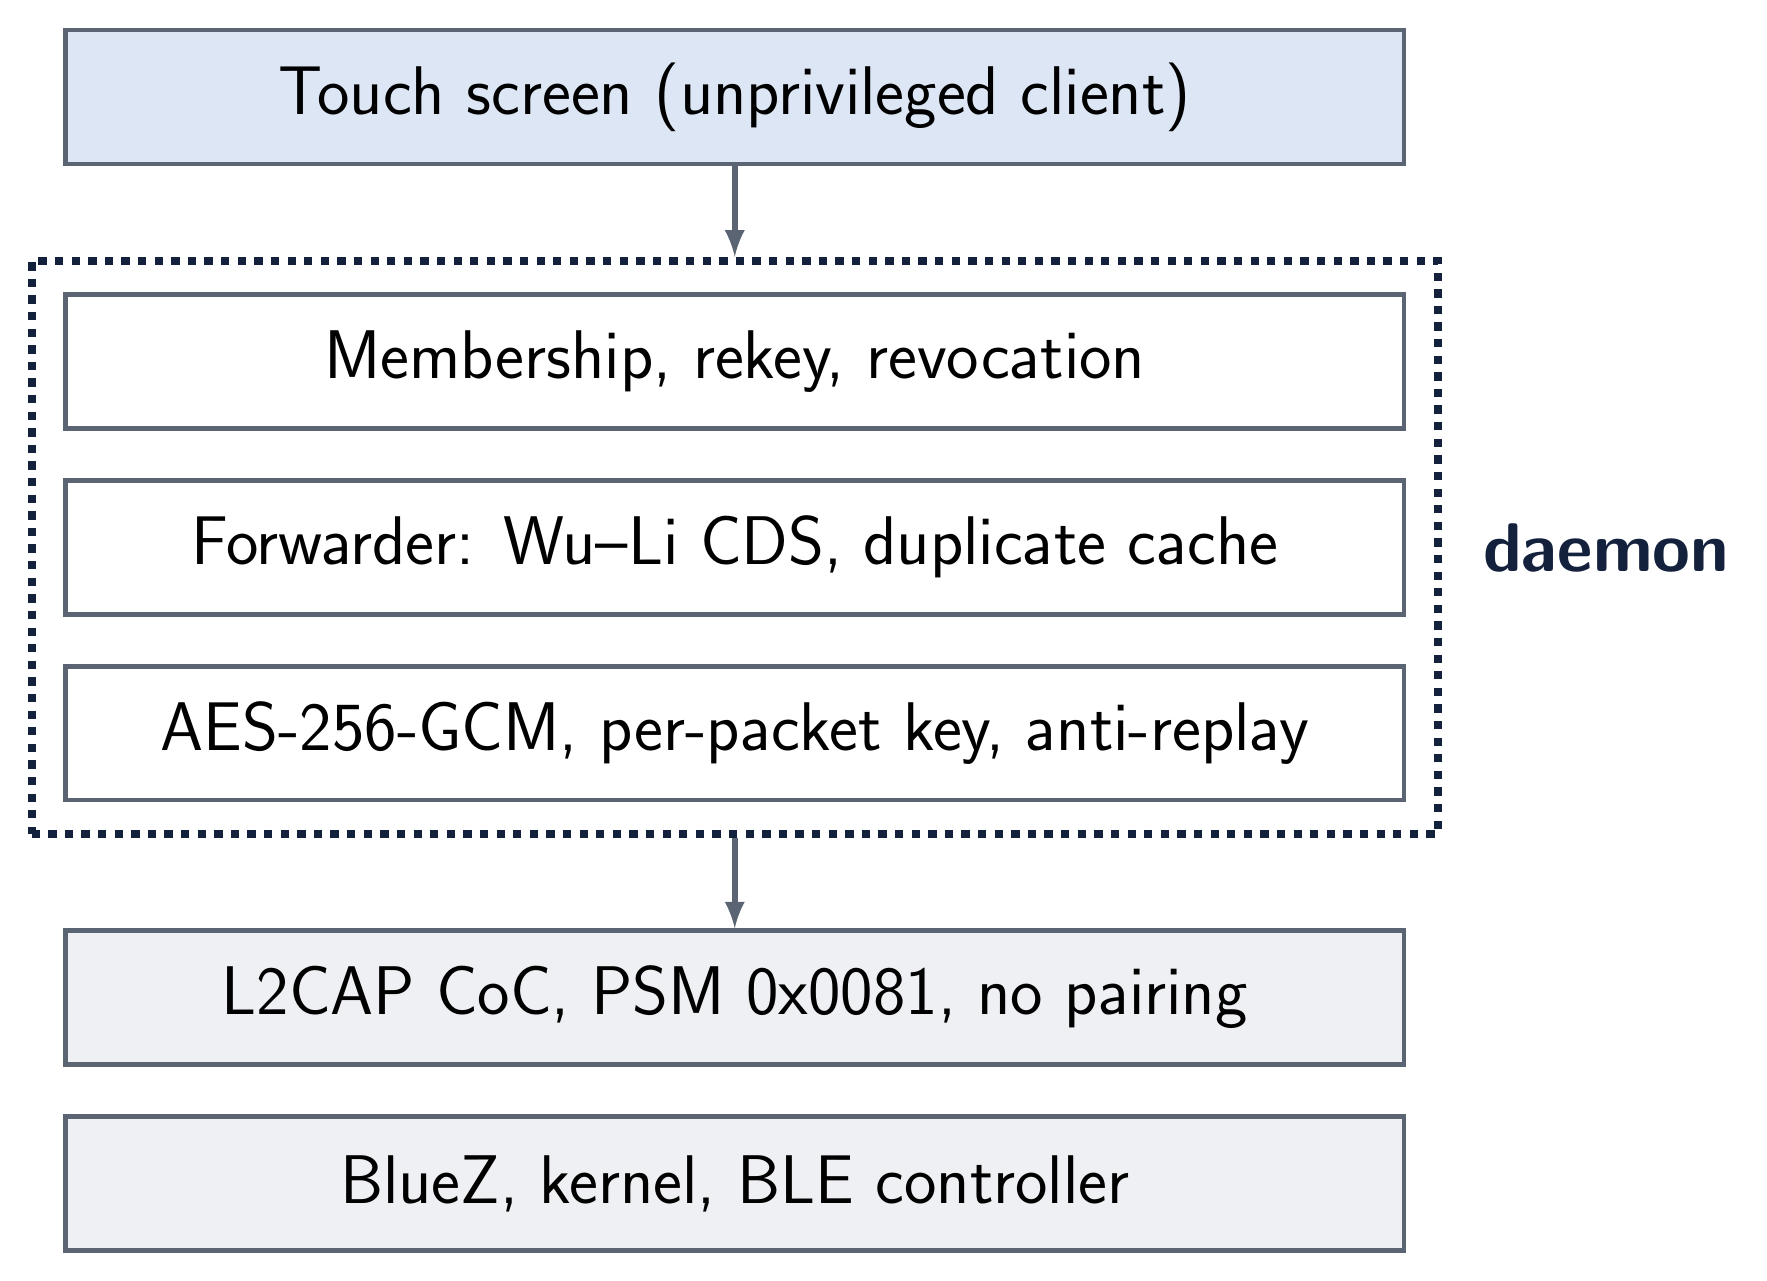
\begin{tikzpicture}[font=\small, node distance=6mm,
  b/.style={draw=muted, fill=#1, minimum width=170mm, minimum height=17mm, align=center, line width=0.6mm},
  b/.default=white]
  \node[b=scr] (ui) {Touch screen (unprivileged client)};
  \node[b, below=16mm of ui] (mem) {Membership, rekey, revocation};
  \node[b, below=of mem] (fwd) {Forwarder: Wu--Li CDS, duplicate cache};
  \node[b, below=of fwd] (sec) {AES-256-GCM, per-packet key, anti-replay};
  \node[b=hdr, below=16mm of sec] (l2) {L2CAP CoC, PSM 0x0081, no pairing};
  \node[b=hdr, below=of l2] (bz) {BlueZ, kernel, BLE controller};
  \node[draw=navy, line width=1mm, dashed, inner sep=4mm, fit=(mem)(sec)] (d) {};
  \node[anchor=west, text=navy, font=\small\bfseries, align=left] at ([xshift=4mm]d.east) {daemon};
  \draw[-latex, line width=0.8mm, muted] (ui) -- (d.north -| ui);
  \draw[-latex, line width=0.8mm, muted] (d.south -| l2) -- (l2);
\end{tikzpicture}
\end{center}
\fig{Figure 1. One daemon per board owns the radio; screens are clients.}

\begin{itemize}
  \item \textbf{Links.} A board advertises an anonymous identifier, a
        relay flag and its L2CAP address. Neighbours open a channel at
        security level \emph{low}: no pairing, no bond.
  \item \textbf{Relays.} Each board applies the Wu--Li rule [7] to its
        two-hop view. The marked boards form a connected dominating set,
        the only ones to rebroadcast.
  \item \textbf{Frames.} Relays read and rewrite only the clear header;
        duplicates are dropped on (source, sequence).
\end{itemize}

\begin{center}
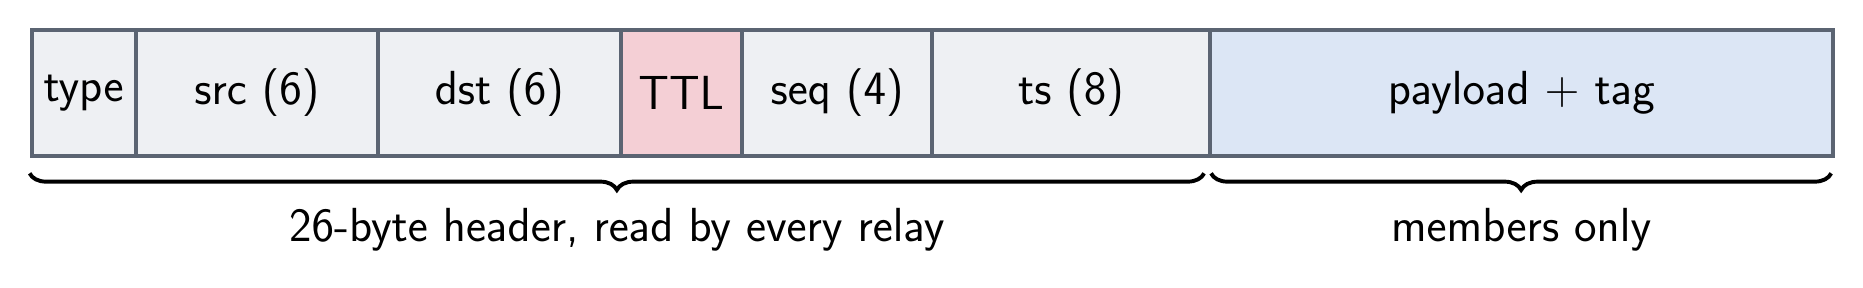
\begin{tikzpicture}[font=\fontsize{19}{23}\selectfont, x=2.2mm, y=1mm,
  f/.style={draw=muted, line width=0.5mm, minimum height=16mm, inner sep=0pt, anchor=south west}]
  \foreach \x/\w/\t/\c in {0/6/type/hdr, 6/14/src (6)/hdr, 20/14/dst (6)/hdr,
                           34/7/TTL/accent!20, 41/11/seq (4)/hdr, 52/16/ts (8)/hdr}
    \node[f, fill=\c, minimum width=\w*2.2mm] at (\x,0) {\t};
  \node[f, fill=scr, minimum width=36*2.2mm] at (68,0) {payload + tag};
  \draw[decorate, decoration={brace, amplitude=6pt, mirror}, line width=0.5mm] (0,-2) -- (67.8,-2)
    node[midway, below=3mm] {26-byte header, read by every relay};
  \draw[decorate, decoration={brace, amplitude=6pt, mirror}, line width=0.5mm] (68.2,-2) -- (104,-2)
    node[midway, below=3mm] {members only};
\end{tikzpicture}
\end{center}
\fig{Figure 2. Frame format; sizes in bytes.}

\sect{At the stand}
\fcolorbox{navy}{scr!45}{\begin{minipage}{0.94\linewidth}\vspace{3mm}
Six boards: three Thundercomm RUBIK Pi 3 screens (Qualcomm QCS6490) and
three Arduino UNO Q relays (Qualcomm QRB2210). Things to try:
\begin{itemize}
  \item send from one screen: the message crosses a relay that is not
        in the group;
  \item exclude a screen or a relay: it keeps relaying, and the next
        message no longer appears on it;
  \item restart the mesh: watch the links and the group come back.
\end{itemize}\vspace{3mm}
\end{minipage}}
\end{minipage}%
\hspace{20mm}%
% ================================================================ column 2
\begin{minipage}[t][935mm][t]{245mm}
\firstsect{3\enspace Security}
\textbf{What each party learns.}\par
{\small
\begin{tabularx}{\linewidth}{@{}X>{\centering\arraybackslash}p{40mm}>{\centering\arraybackslash}p{40mm}>{\centering\arraybackslash}p{34mm}@{}}
\toprule
 & radio listener & relay, not a member & member \\
\midrule
sender and destination address & yes & yes & yes \\
hops left, sequence, time & yes & yes & yes \\
size and timing of traffic & yes & yes & yes \\
text of the message & no & no & \textbf{yes} \\
forge or alter a message & no & no & yes \\
\bottomrule
\end{tabularx}}
\fig{Table 1. Payload privacy, not metadata privacy: the Bluetooth address
is stable and the header is in clear.}

\textbf{Keys.}\par
\begin{center}
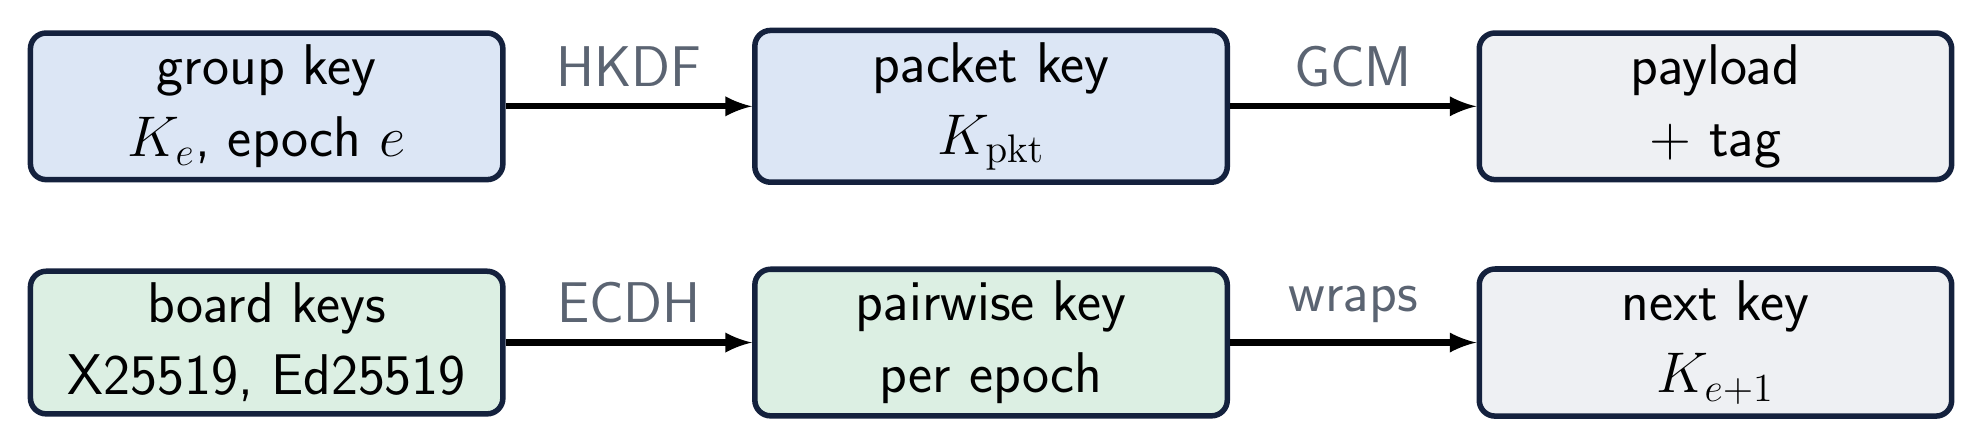
\begin{tikzpicture}[font=\fontsize{21}{26}\selectfont,
  k/.style={draw=navy, line width=0.7mm, fill=#1, rounded corners=2mm, minimum width=60mm, minimum height=17mm, inner sep=1.5mm, align=center},
  k/.default=scr, a/.style={-latex, line width=0.8mm}, lab/.style={above=1mm, text=muted}]
  \node[k] (g) at (0,0) {group key\\$K_e$, epoch $e$};
  \node[k] (p) at (92mm,0) {packet key\\$K_{\mathrm{pkt}}$};
  \node[k=hdr] (f) at (184mm,0) {payload\\+ tag};
  \draw[a] (g) -- node[lab]{HKDF} (p);
  \draw[a] (p) -- node[lab]{GCM} (f);
  \node[k=rel] (x) at (0,-30mm) {board keys\\X25519, Ed25519};
  \node[k=rel] (w) at (92mm,-30mm) {pairwise key\\per epoch};
  \node[k=hdr] (n) at (184mm,-30mm) {next key\\$K_{e+1}$};
  \draw[a] (x) -- node[lab]{ECDH} (w);
  \draw[a] (w) -- node[lab]{wraps} (n);
\end{tikzpicture}
\end{center}
\fig{Figure 3. Top: every frame gets its own key from (source, sequence,
time), so a zero GCM nonce is never reused; the header is authenticated
as associated data, except TTL, which relays decrement. Bottom: each board
floods an Ed25519-signed ANNOUNCE every 30\,s binding its address to its
public keys; pairwise keys carry the next group key.}

\textbf{Removing a member, step by step.}
\begin{enumerate}[label=\arabic*., leftmargin=10mm]
  \item The coordinator is the member with the smallest anonymous
        identifier; every board computes it locally.
  \item It draws $K_{e+1}$ and signs (epoch, $K_{e+1}$, revoked keys)
        with Ed25519.
  \item It wraps that message for every remaining member under their
        pairwise key, skipping the excluded one, and floods it once.
  \item Each member checks the signature, that the signer is the
        coordinator, and that the epoch increases, then switches key.
\end{enumerate}
The excluded board still relays the new traffic; it cannot read it. A
newcomer can be excluded only once its keys have been announced: wait
one ANNOUNCE period after a join.

\textbf{What we accept in this prototype.}\par
{\small
\begin{tabularx}{\linewidth}{@{}>{\raggedright\arraybackslash}p{60mm}>{\raggedright\arraybackslash}X@{}}
\toprule
Who & What it can still do \\
\midrule
Non-member relay & drop or delay frames, rewrite TTL. \\
Active outsider & flood junk; pre-empt a (source, sequence) pair in relay caches. \\
Rogue member & grind its identifier to become coordinator. \\
Observer of a rekey & count the remaining members (one case each). \\
\bottomrule
\end{tabularx}}
\fig{Table 2. Availability attacks remain; confidentiality and authenticity
of the payload do not depend on any relay.}

\textbf{Checked.} On the boards, an excluded screen did not display the
next message (2 trials of 2). In simulation, from 6 to 30 nodes, no
remaining member was stranded and nothing leaked to the excluded one.
\end{minipage}%
\hspace{20mm}%
% ================================================================ column 3
\begin{minipage}[t][935mm][t]{245mm}
\firstsect{4\enspace Four hops across a building}
The stand fits on a table. Spread through the building, about 15\,m
apart with one relay off, the boards formed a line by themselves.

\vspace{6mm}
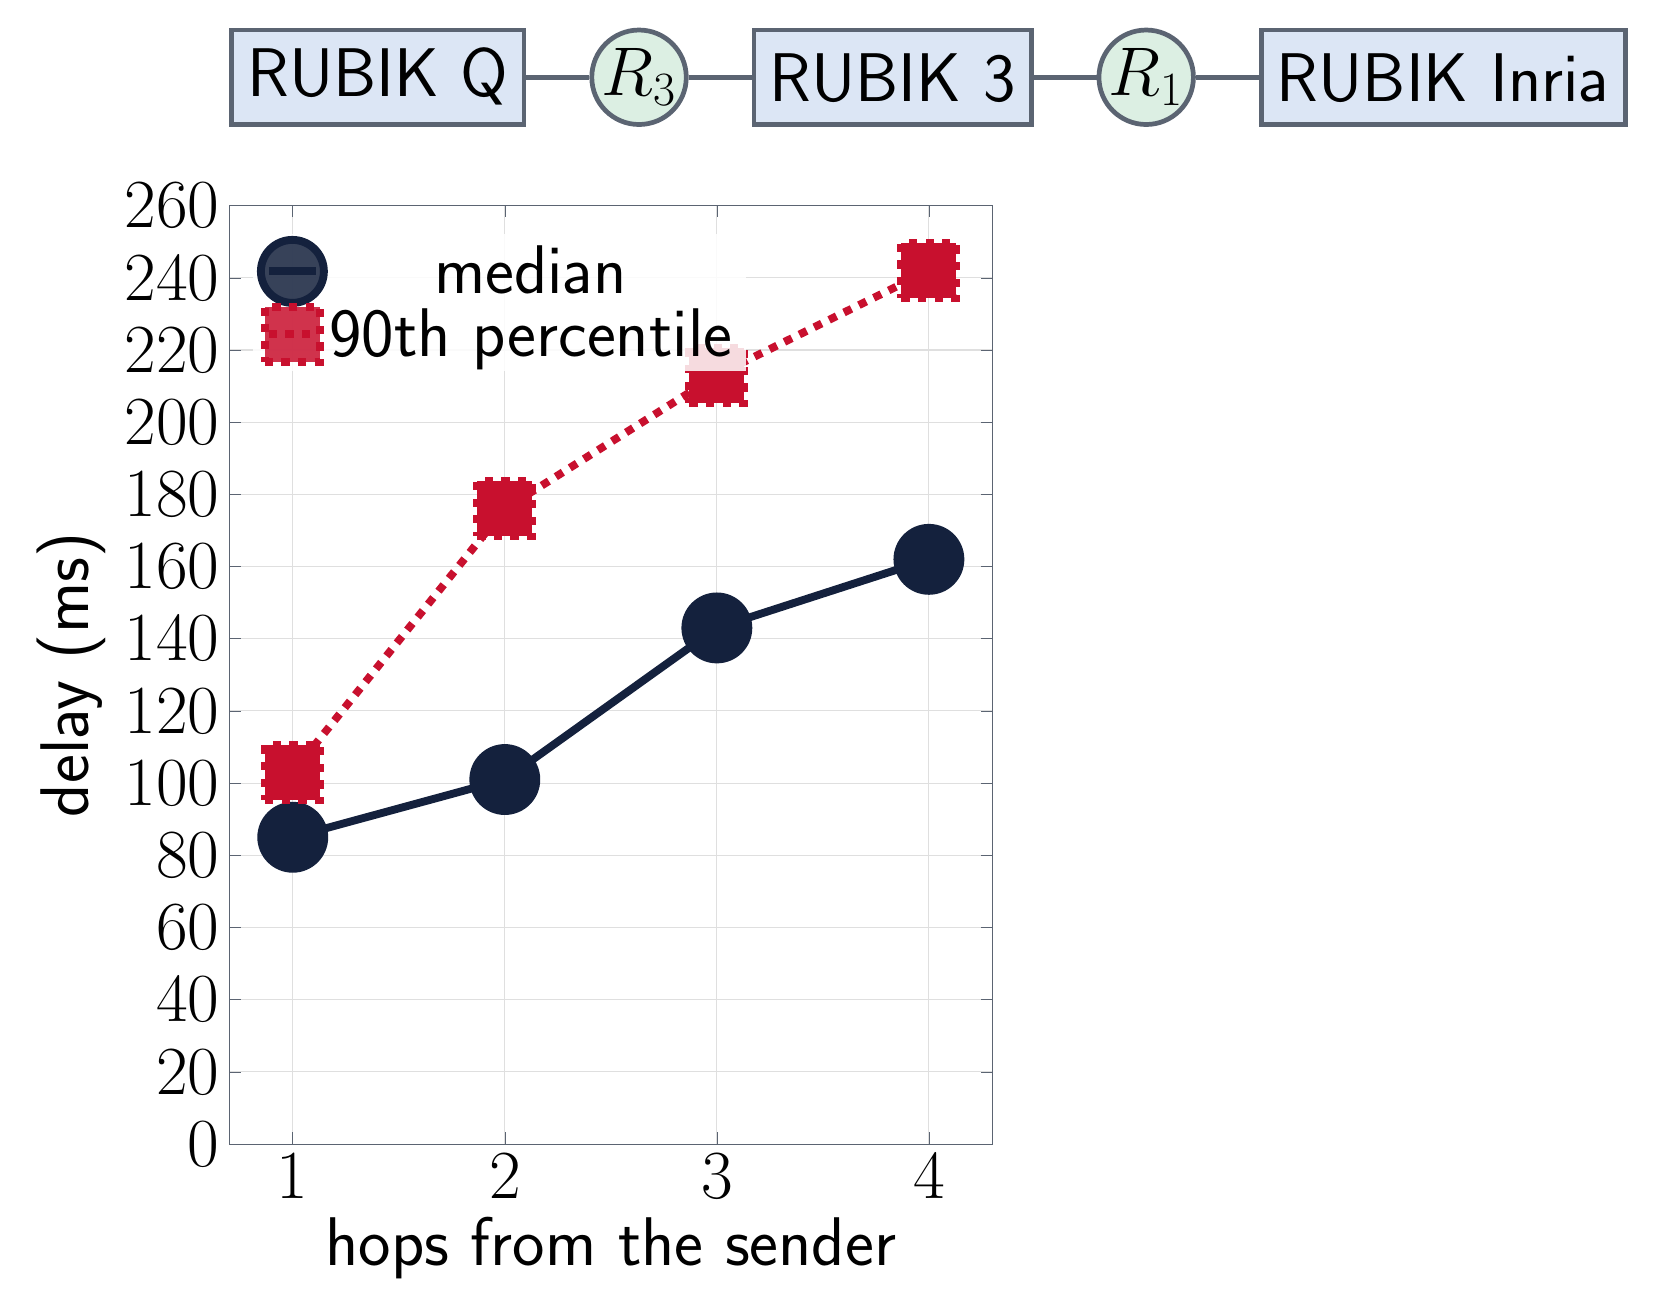
\begin{tikzpicture}[
  s/.style={draw=muted, line width=0.6mm, fill=scr, minimum height=12mm, inner sep=2mm, font=\small},
  r/.style={draw=muted, line width=0.6mm, circle, fill=rel, minimum size=12mm, inner sep=0pt, font=\small}]
\begin{axis}[height=135mm, xlabel={hops from the sender}, ylabel={delay (ms)},
  xmin=0.7, xmax=4.3, ymin=0, ymax=260, xtick={1,2,3,4}, legend pos=north west]
\addplot[line width=1mm, mark=*, mark size=4mm, navy] coordinates {(1,85) (2,101) (3,143) (4,162)};
\addlegendentry{median}
\addplot[line width=1mm, dashed, mark=square*, mark size=3.5mm, accent] coordinates {(1,103) (2,176) (3,213) (4,242)};
\addlegendentry{90th percentile}
\end{axis}
\node[s, anchor=south west] (a) at ([yshift=10mm]current axis.north west) {RUBIK Q};
\node[r, right=8mm of a] (b) {$R_3$};
\node[s, right=8mm of b] (c) {RUBIK 3};
\node[r, right=8mm of c] (d) {$R_1$};
\node[s, right=8mm of d] (e) {RUBIK Inria};
\foreach \u/\v in {a/b,b/c,c/d,d/e} \draw[line width=0.6mm, muted] (\u)--(\v);
\end{tikzpicture}
\fig{Figure 4. Send-to-display delay, on-board clocks within 50\,ms. The far
end received 76 of 79 messages, missing only those sent while the line
formed. Carried away, its link held to about 30\,m.}

\sect{5\enspace 8.2 hours on battery}
The stand on battery, one message every 30\,s: 988 messages, 4\,915
expected receptions.

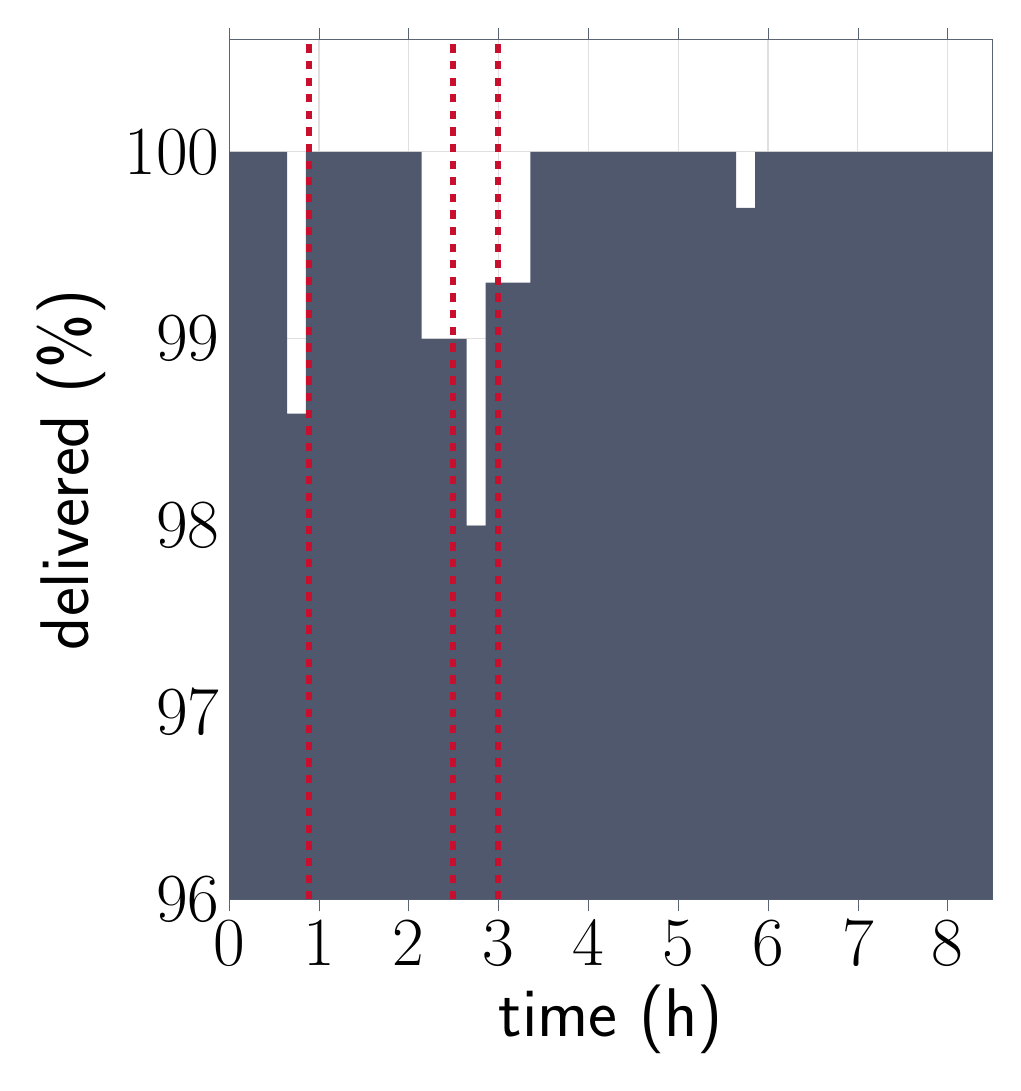
\begin{tikzpicture}
\begin{axis}[height=125mm, xlabel={time (h)}, ylabel={delivered (\%)},
  xmin=0, xmax=8.5, ymin=96, ymax=100.6, xtick={0,1,...,8}, ytick={96,97,98,99,100},
  ybar, bar width=9mm, bar shift=0pt]
\addplot[fill=navy!75, draw=none] coordinates {(0.25,100) (0.75,98.6) (1.25,100) (1.75,100)
  (2.25,99.0) (2.75,98.0) (3.25,99.3) (3.75,100) (4.25,100) (4.75,100) (5.25,100) (5.75,99.7)
  (6.25,100) (6.75,100) (7.25,100) (7.75,100) (8.12,100)};
\draw[accent, line width=0.8mm, dashed] (axis cs:0.89,96) -- (axis cs:0.89,100.6);
\draw[accent, line width=0.8mm, dashed] (axis cs:2.49,96) -- (axis cs:2.49,100.6);
\draw[accent, line width=0.8mm, dashed] (axis cs:2.99,96) -- (axis cs:2.99,100.6);
\end{axis}
\end{tikzpicture}
\fig{Figure 5. Delivery per 30 minutes. Dashed: a relay's Bluetooth
controller stopped answering and was reloaded without a reboot.}

{\small
\begin{tabularx}{\linewidth}{@{}Xr@{}}
\toprule
Received by the screens / by the relays & 100\,\% / 99.3\,\% \\
Delay, median / 99th percentile & 80 / 188\,ms \\
Boards still up when stopped & 6 of 6 \\
\bottomrule
\end{tabularx}}

\sect{6\enspace Limits and next steps}
\begin{itemize}
  \item A restarted sender restarts its sequence numbers, which the
        receivers' anti-replay windows reject: they must survive a
        restart.
  \item TTL\,10 spans about twenty nodes in simulation; on a line, one
        relay is a single point of failure.
  \item Next: an Android port, and replaying the protocol on the contact
        graph the link logs already record, to see how election and
        revocation behave when people move.
\end{itemize}

\vspace{6mm}
{\fontsize{16}{20}\selectfont\color{muted}
[1] N. Achir, P. Jacquet, BUBBLE-BLUE, arXiv:2509.00967, 2025.
[2] Bluetooth SIG, Mesh Profile 1.0, 2017.
[3] J. Dorsey et al., BitChat, 2025.
[4] M. R. Albrecht et al., Breaking Bridgefy, CT-RSA 2021.
[7] J. Wu, H. Li, connected dominating sets, DIAL-M 1999.
\par\vspace{3mm}
Boards provided by the Qualcomm University Platforms program.\par}
\end{minipage}
\end{document}
